% ============================================================
%  Rozdział 2 — Sprzęt
% ============================================================
\section{Sprzęt}

% ------------------------------------------------------------
\subsection{Kajak i pozycja w kajaku}
% ------------------------------------------------------------

Nazwy części kajaka, których warto się nauczyć (bo często się powtarzają):

\begin{itemize}[leftmargin=1.5em, itemsep=2pt]
  \item \textbf{dziób} — przód
  \item \textbf{rufa} — tył
  \item \textbf{kokpit} — otwór wejściowy
  \item \textbf{podnóżek} — oparcie na stopy
  \item \textbf{boczki} — przylegają do bioder
  \item \textbf{motylki} — przylegają do wewnętrznej strony kolan
  \item \textbf{oparcie}
\end{itemize}

\begin{figure}[h]
    \centering
    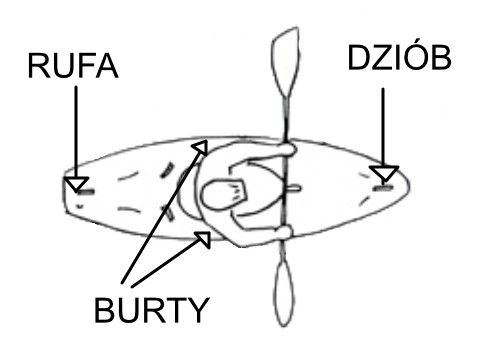
\includegraphics[width=200px]{images/schemat_budowy_kajaka.jpg}
    \caption{Schemat budowy kajaka z opisanymi częściami}
\end{figure}

\textbf{Pozycja.}
Kajakarz siedzi na „żabę" — stopy powinny całą powierzchnią opierać się o podnóżek.Podnóżek musi być solidny, najczęściej wykonany z płyty aluminiowej bądź tworzywa, czasami z pianki wypełniającej cały dziób. Należy zwrócić uwagę, że bardzo niebezpieczne jest wpadnięcie stopy za podnóżek - musi być on tak dopasowany, aby było to absolutnie niemożliwe.

\begin{figure}[h]
    \centering
    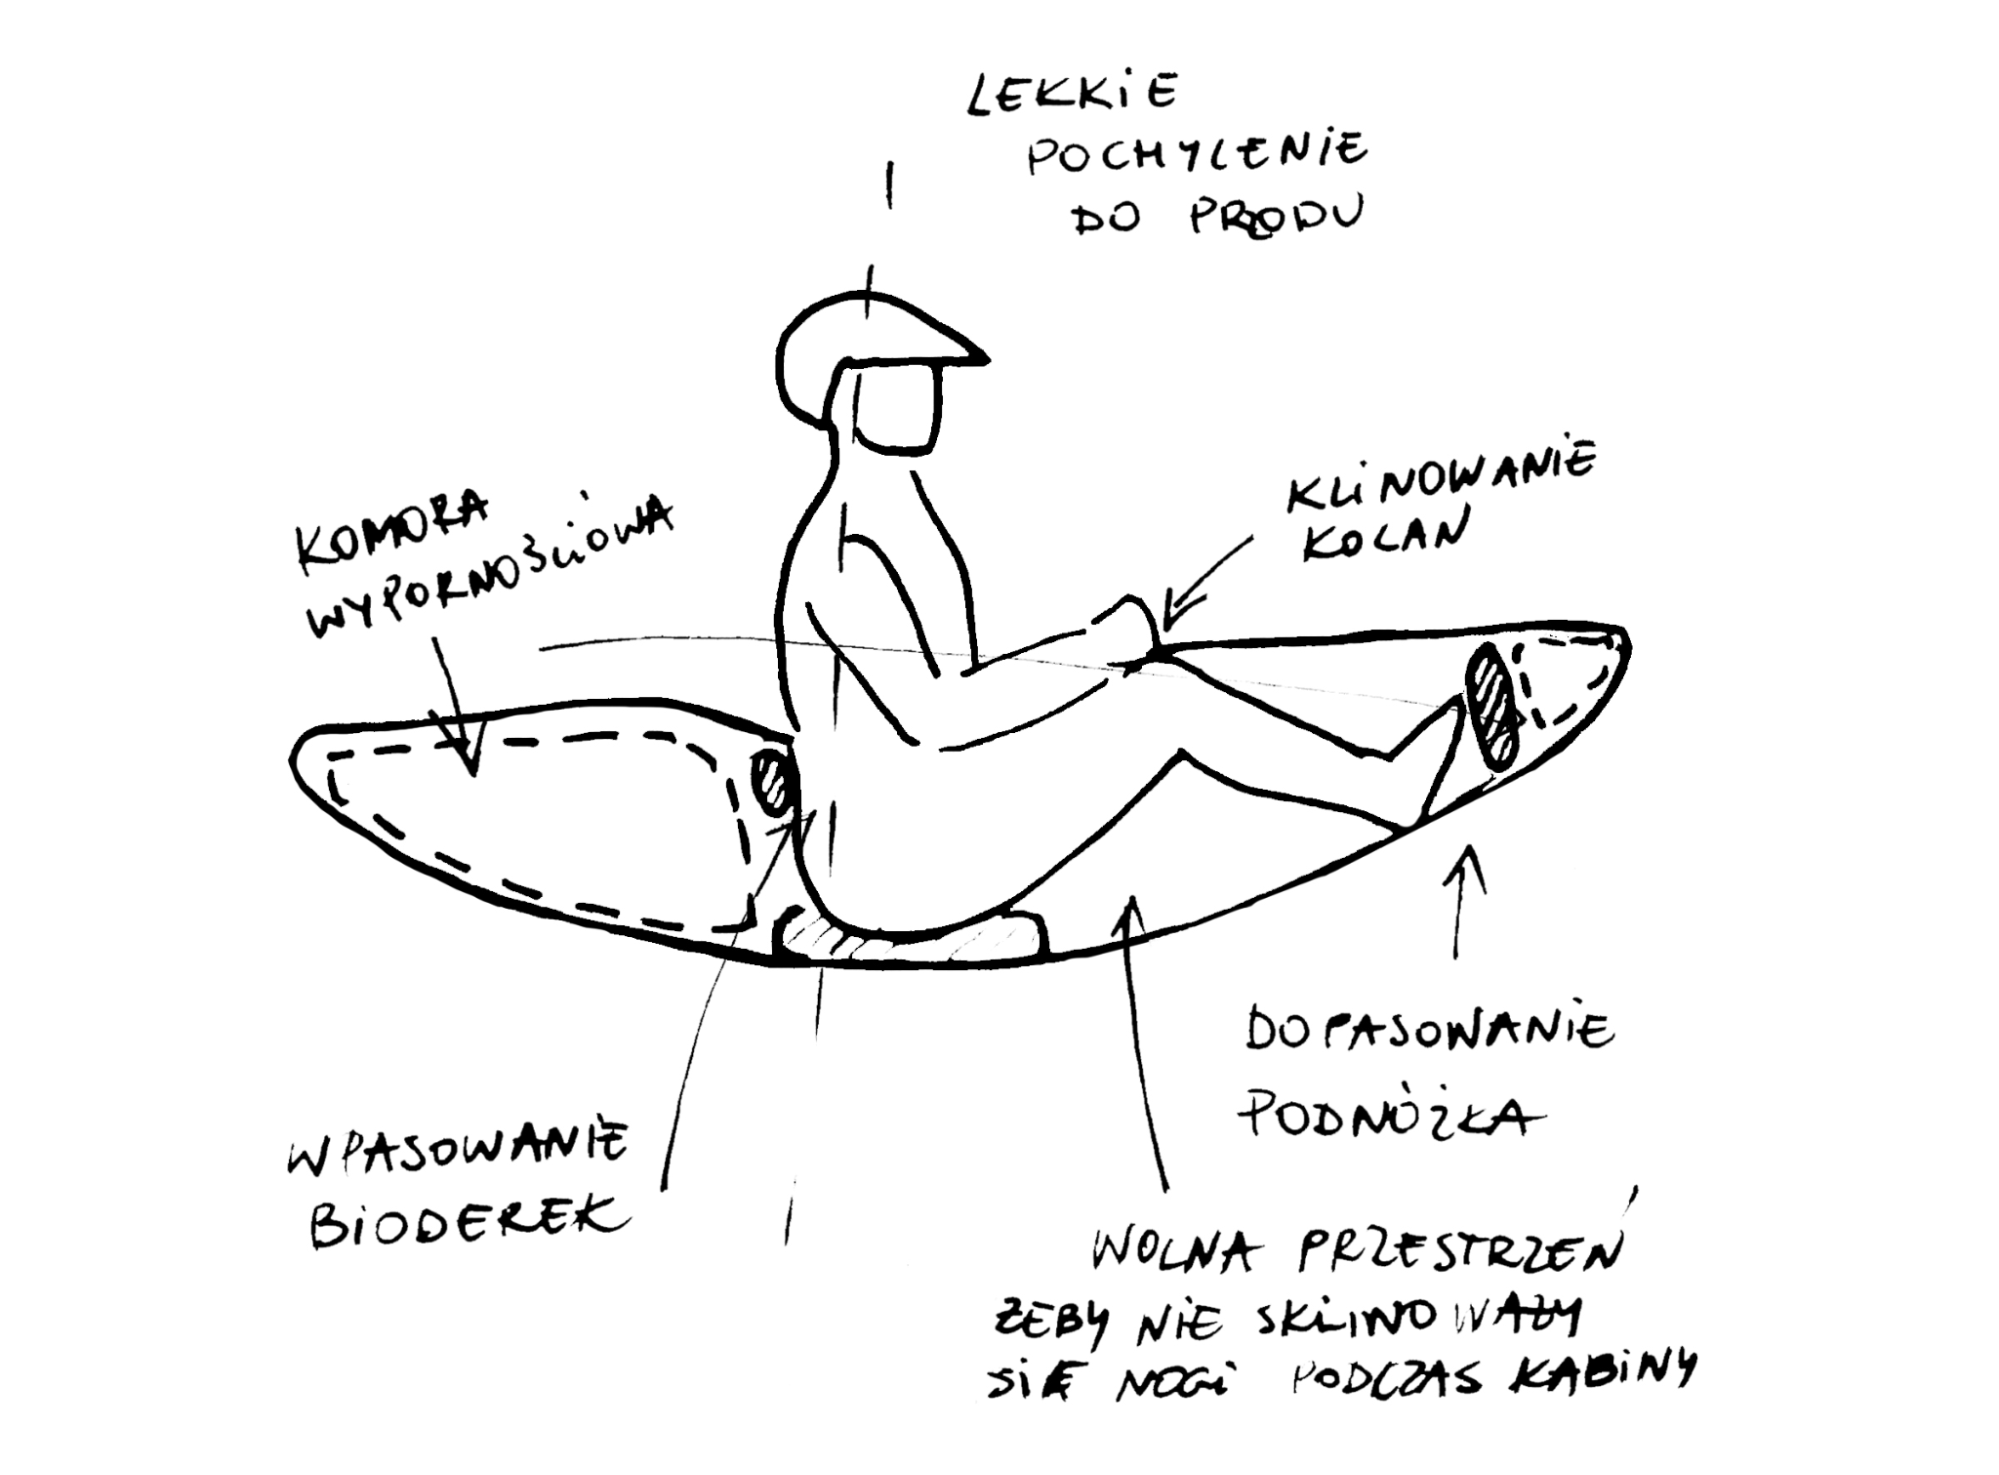
\includegraphics[width=300px]{images/pozycja_w_kajaku.png}
    \caption{Pozycja w kajaku}
\end{figure}

Oparcie służy do wsparcia pozycji na lędźwiach, ale nie opieramy się o nie całym ciężarem; w pozycji aktywnej oparcie powinno dotykać tylko pleców, nie naciskać na nie. Kolana oparte o \emph{motylki} (nakolanniki na burtach) pomagają sterować kajakiem. Biodra powinny mieścić się w siedzeniu i być z obu stron podparte boczkami przylegającymi całą powierzchnią do bioder. Pozycja powinna być neutralna — ciasno, ale komfortowo. Kolana wciskamy w górę w motylki, co daje większą kontrolę nad łódką. Drętwienie nóg i innych części ciała nie jest pożądane.

\begin{tipbox}
  \textbf{Safety box.} Trzymając wiosło, staraj się, aby kąty proste powstałe w łokciach i w obręczy barkowej utrzymywały się podczas manewrów — należy je wykonywać, balansując całą górną częścią ciała, a nie tylko zgięciem w łokciu. Wyobraź sobie, że przed sobą trzymasz pudło i razem z nim poruszasz tułowiem. Taka pozycja stabilizuje obręcz barkową i zabezpiecza przed zwichnięciem oraz wybiciem barków.
\end{tipbox}

\begin{figure}[h]
    \centering
    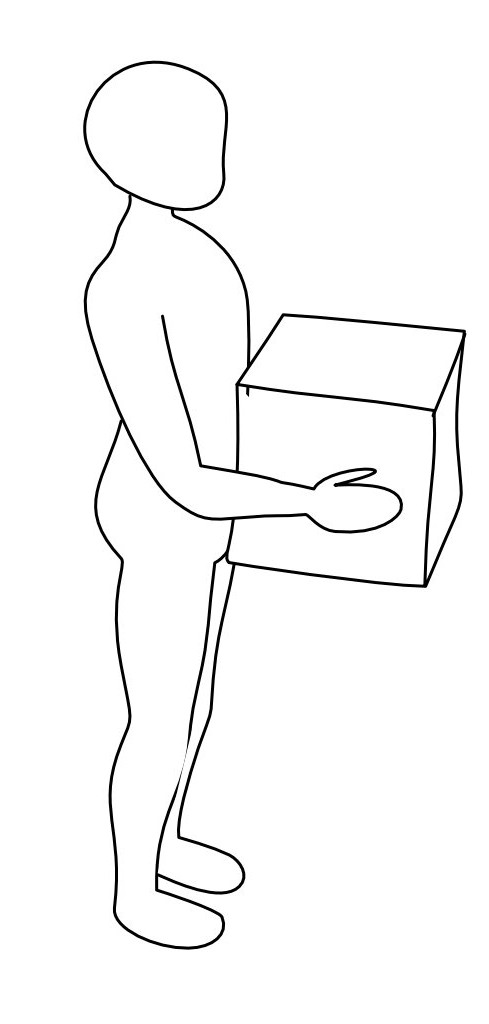
\includegraphics[width=100px]{images/safety_box.jpg}
    \caption{Wizualizacja zasady safety box}
\end{figure}


% ------------------------------------------------------------
\subsection{Rodzaje kajaków}
% ------------------------------------------------------------

Jest wiele rodzajów kajaków (m.in.\ nizinne/zwałkowe, packrafty, slalom, kanadyjki i inne), jednak skupmy się na tych, które będą nas głównie interesować jako kajakarzy pływających docelowo po górach i torach kajakowych.

\begin{description}[leftmargin=1.5em, style=nextline, font=\bfseries]

  \item[Creek]
    Kajak do trudnych, stromych rzek górskich. Duża wyporność, zaokrąglony dziób i rufa. Bardzo stabilny, bezpieczny przy wodospadach i progach. Przeznaczony na trudniejsze odcinki.

  \item[River runner]
    Kajak do stromych rzek górskich. Duża wyporność, zaokrąglony dziób i rufa. Szybszy, ale mniej stabilny od typowego creeka.

  \item[Half-slice]
    Kajak pośredni między river runnerem a playboatem. Posiada okrągły dziób z rockerem (zadartym noskiem), ale cienką rufę. Pozwala na triki i zabawę, ale nadal nadaje się na spływy górskie. Popularny wśród zaawansowanych kajakarzy.

  \item[Playboat / Freestyle]
    Kajak do trików i zabawy w falach oraz odwojach. Krótki i bardzo zwrotny, o małej wyporności, często z płaskim dnem. Raczej nie nadaje się do pływania w górach;na torze kajakowym może się sprawdzić. Nie nadaje się na długie spływy.

  \item[Full-slice]
    Kajak o małej wyporności na całej długości. Bardzo reaktywny i techniczny — idealny do freestyle'u i zabawy. Wymaga dużych umiejętności.

\end{description}

\subsubsection*{Kryteria doboru kajaka}

\begin{description}[leftmargin=1.5em, font=\bfseries]
  \item[Cel]
    Dobieramy kajak odpowiednio do swoich umiejętności, poziomu trudności akwenu i elementów, które będziemy ćwiczyć. Inny kajak wybierzemy na trudną rzekę górską, inny na tor kajakowy, a jeszcze inny na płaską wodę.

  \item[Waga kajakarza]
    Warto stosować się do zakresu wagowego kajaka — ma to wpływ na bezpieczeństwo, zanurzenie łódki, wyporność i stabilność. Przekroczenie wagi prowadzi do utraty stabilności i zwiększa ryzyko wywrotki; zbyt duży kajak jest mniej sterowny i wymaga więcej siły. Wybór zbyt dużego kajaka utrudnia też naukę i oswajanie się
    z wywrotkami.
\end{description}

% ------------------------------------------------------------
\subsection{Wiosło}
% ------------------------------------------------------------

Wiosło składa się z \textbf{dwóch piór} (strona pasywna — wypukła; strona aktywna — wklęsła) oraz \textbf{drążka}.

\textbf{Długość.}
Odpowiednia długość wiosła odpowiada mniej więcej wysokości nadgarstka kajakarza z ręką wyciągniętą do góry (z uwzględnieniem indywidualnych preferencji). Im dłuższe wiosło, tym trudniejsze może być wiosłowanie; jednak dla wysokich osób lub szerokiego kajaka jest ono wskazane. Krótszym wiosłem można wiosłować bardziej agresywnie i pionowo.

\begin{figure}[h]
    \centering
    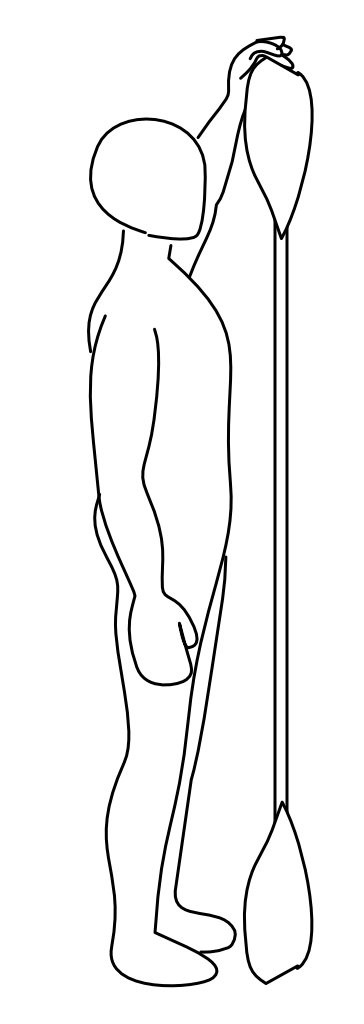
\includegraphics[width=80px]{images/dlugosc_wiosla.jpg}
    \caption{Przyklad metody dobioru dlugości wiosła}
\end{figure}

\textbf{Rotacja pióra.}
Zapewnia komfort i efektywność podczas wiosłowania. Przy wiosłach skrętnych ruch nadgarstków jest bardziej ergonomiczny, co pomaga podczas dłuższych spływów. W kajakarstwie górskim najczęściej spotykane są kąty w okolicach 30-45°. Wiosła proste są głównie wykorzystywane we freestyle'u, gdzie symetria ruchów po obu stronach jest kluczowa.

% ------------------------------------------------------------
\subsection{Fartuch}
% ------------------------------------------------------------

Komin fartucha nakładamy na ciało na wysokości pasa (może sięgać nawet do klatki piersiowej). Gumę na obwodzie zakłada się na kokpit kajaka — fartuch zapobiega wlewaniu się wody do kajaka. Dobrze dobrany fartuch powinniśmy móc samodzielnie założyć na kajak oraz zerwać go w przypadku konieczności szybkiego opuszczenia kajaka. 

Rozmiar \textbf{pokładu} fartucha musi być dopasowany do rozmiaru kokpitu kajaka, a rozmiar \textbf{komina} — do obwodu w pasie.

\begin{tipbox}
  Mokry neopren łatwiej się rozciąga — jeśli masz problem z naciągnięciem fartucha na kokpicie, zamocz fartuch przed założeniem.
\end{tipbox}

% ------------------------------------------------------------
\subsection{Kask}
% ------------------------------------------------------------

Kask powinien być dobrze dopasowany do głowy — nie poruszać się przy potrząsaniu głową, nawet gdy jesteśmy pochyleni. Chroni przed stłuczeniami i urazami spowodowanymi uderzeniem o skałę, wiosło współtowarzyszy lub krawędź basenu.

Pasek zapinamy \textbf{zawsze} — nawet na lądzie. Wyrobieniu tego nawyku służy konsekwentne zapinanie kasku poza wodą. Pasek powinien być ciasny, ale nie utrudniać oddychania.

\begin{tipbox}
  Każda firma ma własny zakres rozmiarów, który nie gwarantuje idealnego dopasowania. Przed wyjazdem warto przymierzyć kask klubowy, a przed zakupem własnego pożyczyć go na próbę od znajomych.
\end{tipbox}

% ------------------------------------------------------------
\subsection{Kamizelka}
% ------------------------------------------------------------

\textbf{Kamizelki górskie} mają dużą wyporność pozwalającą na utrzymanie kajakarza na powierzchni rwącej wody. Mają wbudowany pas przystosowany do wpięcia podczas akcji ratunkowej (z możliwością szybkiego wypięcia), liczne kieszenie i uchwyty. Pomimo rozbudowanej konstrukcji zapewniają dużą swobodę ruchów.

Na rzekach nizinnych wystarczająca jest \textbf{kamizelka nizinna} — mniej wyporna, ale ze względu na prostszą konstrukcję mniej ograniczająca ruchy przy pokonywaniu zwałek.

% ------------------------------------------------------------
\subsection{Rzutka}
% ------------------------------------------------------------

Miękka, mocna lina o jaskrawym kolorze, unosząca się na wodzie, znajdująca się w worku. Główne zastosowanie: rzucanie w celu wyłowienia osoby znajdującej się w wodzie. Dostępna w długościach 10-35\,m (dobieramy w zależności od potrzeb i umiejętności rzucającego). Rzutka powinna być zawsze dobrze \textbf{sklarowana} (ułożona w worku).
i gotowa do użycia.

\begin{warnbox}
  Na rzece górskiej należy \textbf{ZAWSZE} mieć rzutkę przy sobie — nawet gdy wychodzimy z kajaka obserwując rzekę z brzegu. Używając liny, zawsze warto mieć przy sobie \textbf{nóż}.
\end{warnbox}

% ------------------------------------------------------------
\subsection{Komory}
% ------------------------------------------------------------

Komory służą do wypełnienia kajaka powietrzem. Nie poprawiają wyporności kajaka, natomiast dzięki nim kajak nabiera mniejszą ilość wody po kabinie, co znacznie ułatwia jego wyłowienie.

Komory występują zazwyczaj w rozmiarach:

\begin{itemize}[leftmargin=1.5em]
  \item \textbf{20\,L} — wsadza się na tył kajaka (zazwyczaj dwie, jeśli przez środekprzebiega przegroda)
  \item \textbf{10\,L} — wsadza się na przód kajaka, jeśli za podnóżkiem jest miejsce
\end{itemize}

% ------------------------------------------------------------
\subsection{Ubiór kajakarza i lista rzeczy na spływ}
% ------------------------------------------------------------

\begin{tabular}{>{\bfseries}p{3cm} p{10cm}}
\toprule
\textbf{Kategoria} & \textbf{Wyposażenie} \\
\midrule

Basen &
\begin{itemize}[leftmargin=*, nosep, topsep=0pt]
  \item Kąpielówki przylegające
  \item Nosek
  \item Zatyczki do uszu*
  \item Klapki
  \item Okularki (opcjonalnie)
  \item Ręcznik
\end{itemize} \\
\midrule

Pływanie &
\begin{itemize}[leftmargin=*, nosep, topsep=0pt]
  \item Obuwie do wody / neoprenowe (wiązane, grubsza podeszwa)
  \item Czapka z daszkiem / kapelusz / bandana
  \item Krem z filtrem
  \item Bidon
  \item Wodoodporny worek z suchymi ubraniami
  \item Nosek, zatyczki do uszu (opcjonalne)
  \item Ubranie dopasowane do pogody (neopren / polar / kurtka pół-sucha lub sucha)
\end{itemize} \\
\midrule

Biwak &
\begin{itemize}[leftmargin=*, nosep, topsep=0pt]
  \item Namiot
  \item Karimata
  \item Śpiwór
  \item Odzież: polar, neopren lub wełna
  \item Ciepłe nakrycie głowy
  \item Płaszcz przeciwdeszczowy
  \item Latarka / czołówka
  \item Menażka, kubek, sztućce
  \item Spray na komary
  \item \textbf{Dobry humor :)}
\end{itemize} \\
\midrule

Dodatkowo &
\begin{itemize}[leftmargin=*, nosep, topsep=0pt]
  \item Krem z filtrem
  \item Pomadka nawilżająca
  \item Krzesełko turystyczne
  \item Instrument muzyczny
  \item Nóż składany
  \item Apteczka
  \item Taśma z karabinkiem
  \item Bidon z wodą
\end{itemize} \\
\bottomrule
\end{tabular}